\section{Problema 4}
Supongamos que hay 4 líneas de buses entre A y B; y 3 líneas de buses entre B y C. ¿De cuántas maneras puede una persona viajar en viaje redondo (ida y vuelta) de A a C, sin usar ninguna línea de bus más de una vez?

\begin{solution}
Visualicemos el problema: 
\begin{center}
    

\tikzset{every picture/.style={line width=0.75pt}} %set default line width to 0.75pt        

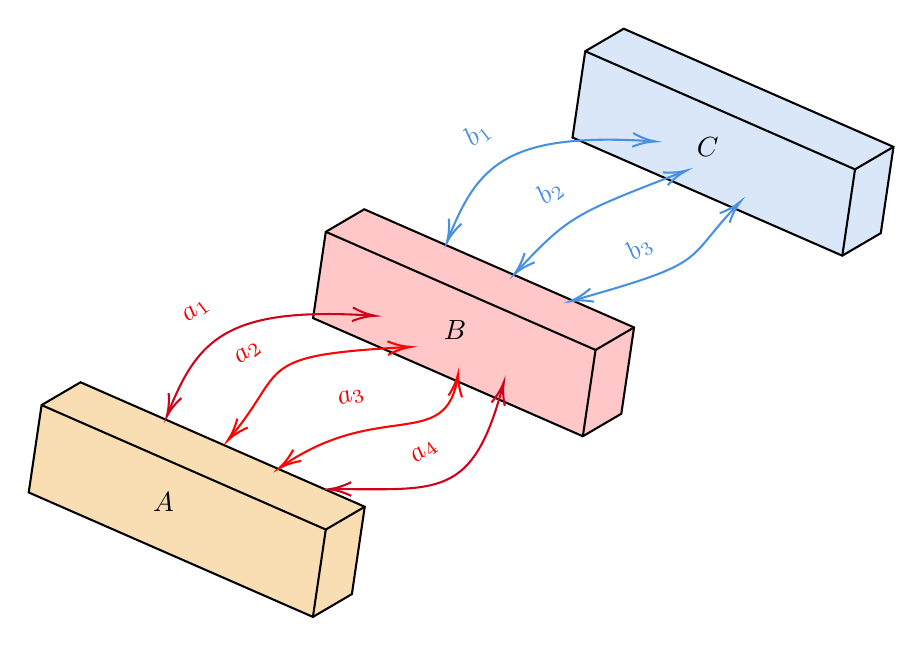
\begin{tikzpicture}[x=0.75pt,y=0.75pt,yscale=-1,xscale=1]
%uncomment if require: \path (0,300); %set diagram left start at 0, and has height of 300

%Shape: Cube [id:dp19630639075995027] 
\draw  [fill={rgb, 255:red, 255; green, 1; blue, 1 }  ,fill opacity=0.22 ] (245.66,99.96) -- (264.2,89.11) -- (394.18,146.03) -- (388.05,187.61) -- (369.51,198.46) -- (239.53,141.54) -- cycle ; \draw   (394.18,146.03) -- (375.64,156.88) -- (245.66,99.96) ; \draw   (375.64,156.88) -- (369.51,198.46) ;
%Shape: Cube [id:dp5121656042070563] 
\draw  [fill={rgb, 255:red, 74; green, 144; blue, 226 }  ,fill opacity=0.21 ] (370.66,12.96) -- (389.2,2.11) -- (519.18,59.03) -- (513.05,100.61) -- (494.51,111.46) -- (364.53,54.54) -- cycle ; \draw   (519.18,59.03) -- (500.64,69.88) -- (370.66,12.96) ; \draw   (500.64,69.88) -- (494.51,111.46) ;
%Shape: Cube [id:dp9223007421491981] 
\draw  [fill={rgb, 255:red, 236; green, 150; blue, 9 }  ,fill opacity=0.31 ] (108.73,183.45) -- (127.5,172.46) -- (264.43,232.43) -- (258.23,274.52) -- (239.46,285.5) -- (102.53,225.54) -- cycle ; \draw   (264.43,232.43) -- (245.66,243.41) -- (108.73,183.45) ; \draw   (245.66,243.41) -- (239.46,285.5) ;
%Curve Lines [id:da9236988327654716] 
\draw [color={rgb, 255:red, 208; green, 2; blue, 27 }  ,draw opacity=1 ]   (169.86,186.83) .. controls (183.9,151.93) and (197.75,135.69) .. (268.36,140.36) ;
\draw [shift={(269.43,140.43)}, rotate = 183.92] [color={rgb, 255:red, 208; green, 2; blue, 27 }  ,draw opacity=1 ][line width=0.75]    (10.93,-3.29) .. controls (6.95,-1.4) and (3.31,-0.3) .. (0,0) .. controls (3.31,0.3) and (6.95,1.4) .. (10.93,3.29)   ;
\draw [shift={(169,189)}, rotate = 291.53] [color={rgb, 255:red, 208; green, 2; blue, 27 }  ,draw opacity=1 ][line width=0.75]    (10.93,-3.29) .. controls (6.95,-1.4) and (3.31,-0.3) .. (0,0) .. controls (3.31,0.3) and (6.95,1.4) .. (10.93,3.29)   ;
%Curve Lines [id:da8519542966027018] 
\draw [color={rgb, 255:red, 255; green, 3; blue, 3 }  ,draw opacity=1 ]   (225.17,212.49) .. controls (271.7,180.74) and (303.54,206.06) .. (309.19,170.11) ;
\draw [shift={(309.43,168.43)}, rotate = 457.31] [color={rgb, 255:red, 255; green, 3; blue, 3 }  ,draw opacity=1 ][line width=0.75]    (10.93,-3.29) .. controls (6.95,-1.4) and (3.31,-0.3) .. (0,0) .. controls (3.31,0.3) and (6.95,1.4) .. (10.93,3.29)   ;
\draw [shift={(223,214)}, rotate = 324.48] [color={rgb, 255:red, 255; green, 3; blue, 3 }  ,draw opacity=1 ][line width=0.75]    (10.93,-3.29) .. controls (6.95,-1.4) and (3.31,-0.3) .. (0,0) .. controls (3.31,0.3) and (6.95,1.4) .. (10.93,3.29)   ;
%Curve Lines [id:da8967339679578482] 
\draw [color={rgb, 255:red, 208; green, 2; blue, 27 }  ,draw opacity=1 ]   (249.34,223.98) .. controls (299.43,223.63) and (316.32,229.44) .. (330.98,174.12) ;
\draw [shift={(331.43,172.43)}, rotate = 464.5] [color={rgb, 255:red, 208; green, 2; blue, 27 }  ,draw opacity=1 ][line width=0.75]    (10.93,-3.29) .. controls (6.95,-1.4) and (3.31,-0.3) .. (0,0) .. controls (3.31,0.3) and (6.95,1.4) .. (10.93,3.29)   ;
\draw [shift={(247,224)}, rotate = 359.38] [color={rgb, 255:red, 208; green, 2; blue, 27 }  ,draw opacity=1 ][line width=0.75]    (10.93,-3.29) .. controls (6.95,-1.4) and (3.31,-0.3) .. (0,0) .. controls (3.31,0.3) and (6.95,1.4) .. (10.93,3.29)   ;
%Curve Lines [id:da8526320801010947] 
\draw [color={rgb, 255:red, 74; green, 144; blue, 226 }  ,draw opacity=1 ]   (304.86,102.83) .. controls (318.9,67.93) and (332.75,51.69) .. (403.36,56.36) ;
\draw [shift={(404.43,56.43)}, rotate = 183.92] [color={rgb, 255:red, 74; green, 144; blue, 226 }  ,draw opacity=1 ][line width=0.75]    (10.93,-3.29) .. controls (6.95,-1.4) and (3.31,-0.3) .. (0,0) .. controls (3.31,0.3) and (6.95,1.4) .. (10.93,3.29)   ;
\draw [shift={(304,105)}, rotate = 291.53] [color={rgb, 255:red, 74; green, 144; blue, 226 }  ,draw opacity=1 ][line width=0.75]    (10.93,-3.29) .. controls (6.95,-1.4) and (3.31,-0.3) .. (0,0) .. controls (3.31,0.3) and (6.95,1.4) .. (10.93,3.29)   ;
%Curve Lines [id:da5716803692726303] 
\draw [color={rgb, 255:red, 74; green, 144; blue, 226 }  ,draw opacity=1 ]   (365.49,132.85) .. controls (431.53,114.17) and (417.17,115.1) .. (444.17,86.74) ;
\draw [shift={(445.43,85.43)}, rotate = 494.03] [color={rgb, 255:red, 74; green, 144; blue, 226 }  ,draw opacity=1 ][line width=0.75]    (10.93,-3.29) .. controls (6.95,-1.4) and (3.31,-0.3) .. (0,0) .. controls (3.31,0.3) and (6.95,1.4) .. (10.93,3.29)   ;
\draw [shift={(363.43,133.43)}, rotate = 344.26] [color={rgb, 255:red, 74; green, 144; blue, 226 }  ,draw opacity=1 ][line width=0.75]    (10.93,-3.29) .. controls (6.95,-1.4) and (3.31,-0.3) .. (0,0) .. controls (3.31,0.3) and (6.95,1.4) .. (10.93,3.29)   ;
%Curve Lines [id:da161419448202348] 
\draw [color={rgb, 255:red, 255; green, 3; blue, 3 }  ,draw opacity=1 ]   (199.75,198.87) .. controls (227.71,165.42) and (209.78,159.43) .. (285.28,155.49) ;
\draw [shift={(286.43,155.43)}, rotate = 537.06] [color={rgb, 255:red, 255; green, 3; blue, 3 }  ,draw opacity=1 ][line width=0.75]    (10.93,-3.29) .. controls (6.95,-1.4) and (3.31,-0.3) .. (0,0) .. controls (3.31,0.3) and (6.95,1.4) .. (10.93,3.29)   ;
\draw [shift={(198.43,200.43)}, rotate = 310.6] [color={rgb, 255:red, 255; green, 3; blue, 3 }  ,draw opacity=1 ][line width=0.75]    (10.93,-3.29) .. controls (6.95,-1.4) and (3.31,-0.3) .. (0,0) .. controls (3.31,0.3) and (6.95,1.4) .. (10.93,3.29)   ;
%Curve Lines [id:da5871528552964772] 
\draw [color={rgb, 255:red, 74; green, 144; blue, 226 }  ,draw opacity=1 ]   (338.02,118.72) .. controls (363.27,91.69) and (366.45,91.02) .. (417.86,71.04) ;
\draw [shift={(419.43,70.43)}, rotate = 518.75] [color={rgb, 255:red, 74; green, 144; blue, 226 }  ,draw opacity=1 ][line width=0.75]    (10.93,-3.29) .. controls (6.95,-1.4) and (3.31,-0.3) .. (0,0) .. controls (3.31,0.3) and (6.95,1.4) .. (10.93,3.29)   ;
\draw [shift={(336.43,120.43)}, rotate = 312.95] [color={rgb, 255:red, 74; green, 144; blue, 226 }  ,draw opacity=1 ][line width=0.75]    (10.93,-3.29) .. controls (6.95,-1.4) and (3.31,-0.3) .. (0,0) .. controls (3.31,0.3) and (6.95,1.4) .. (10.93,3.29)   ;

% Text Node
\draw (161,224.21) node [anchor=north west][inner sep=0.75pt]    {$A$};
% Text Node
\draw (301,141.21) node [anchor=north west][inner sep=0.75pt]    {$B$};
% Text Node
\draw (423,53.21) node [anchor=north west][inner sep=0.75pt]    {$C$};
% Text Node
\draw (173.6,138.87) node [anchor=north west][inner sep=0.75pt]  [color={rgb, 255:red, 244; green, 0; blue, 0 }  ,opacity=1 ,rotate=-322.11]  {$a_{1}$};
% Text Node
\draw (198.6,158.87) node [anchor=north west][inner sep=0.75pt]  [color={rgb, 255:red, 244; green, 0; blue, 0 }  ,opacity=1 ,rotate=-322.11]  {$a_{2}$};
% Text Node
\draw (248.64,177.47) node [anchor=north west][inner sep=0.75pt]  [color={rgb, 255:red, 244; green, 0; blue, 0 }  ,opacity=1 ,rotate=-339.89]  {$a_{3}$};
% Text Node
\draw (283.6,206.87) node [anchor=north west][inner sep=0.75pt]  [color={rgb, 255:red, 244; green, 0; blue, 0 }  ,opacity=1 ,rotate=-322.11]  {$a_{4}$};
% Text Node
\draw (308.6,51.87) node [anchor=north west][inner sep=0.75pt]  [color={rgb, 255:red, 74; green, 144; blue, 226 }  ,opacity=1 ,rotate=-322.11]  {$b_{1}$};
% Text Node
\draw (343.6,79.87) node [anchor=north west][inner sep=0.75pt]  [color={rgb, 255:red, 74; green, 144; blue, 226 }  ,opacity=1 ,rotate=-322.11]  {$b_{2}$};
% Text Node
\draw (386.6,106.87) node [anchor=north west][inner sep=0.75pt]  [color={rgb, 255:red, 74; green, 144; blue, 226 }  ,opacity=1 ,rotate=-322.11]  {$b_{3}$};


\end{tikzpicture}
\end{center}

Es decir, tenemos un problema de combinatoria. Para el tramo $A-B$: 
$$C(4,1)= 4 \text{ formas.}$$
Para el tramo $B-C$: 
$$C(3,1)= 3 \text{ formas.}$$
Ahora de regreso, tramo $C-B$: 
$$C(2,1)= 2 \text{ formas.}$$
Para el tramo $B-A$:
$$C(3,1)= 3 \text{ formas.}$$

Por lo tanto, las maneras que se puede hacer un viaje redondo son (aplicando el principio del producto):
$$C(4,1)\cdot C(3,1)\cdot C(2,1)\cdot  C(3,1)=4\cdot 3 \cdot 2\cdot 3 = 72 \text{ formas.}$$
\end{solution}